% !TEX TS-program = xelatex
\documentclass[FM]{tulpresentation}
\title{Tvorba a využití botu pro výuku matematiky na platformě Discord}
\author{Radek Mocek}
\institute{Ing. Igor Kopetschke}
\newcommand{\authorPhone}{}
\newcommand{\authorMail}{Aplikovaná informatika}
\setbeamertemplate{enumerate items}[default]
\begin{document}
	\TULtitleframe
	
	\begin{frame}\frametitle{Cíle bakalářské práce}
		\begin{enumerate}
			\item Vypracujte rešerši sociálních platforem, které umožňují integraci botů.
			\item Analyzujte vybranou skupinu existujících botů na platformě Discord a knihoven pro jejich tvorbu.
			\item Navrhněte bot zaměřený na výklad a příklady z lineární algebry při využití specifických funkcí Discordu včetně administrace a interaktivních zpráv.
			\item Navržené řešení implementujte a nasaďte do testovacího provozu pro vybranou skupinu uživatelů.
			\item Vyhodnoťte zpětnou vazbu od uživatelů a navrhněte případné úpravy a vylepšení.
		\end{enumerate}
	\end{frame}
	
	\begin{frame}\frametitle{Výsledek bakalářské práce}
		\begin{itemize}
			\item Discord bot implementovaný v jazyce Python
			\begin{itemize}
				\item Knihovny discord.py, Matplotlib, NumPy, SymPy
			\end{itemize}
			\item Tři hlavní funkce v prostředí textového chatu
			\begin{itemize}
				\item Vykreslování matematických výrazů
				\item Výklad teorie
				\item Generace příkladů
			\end{itemize}
			\item Demonstrace specifických vlastností platformy Discord:			
		\end{itemize}
		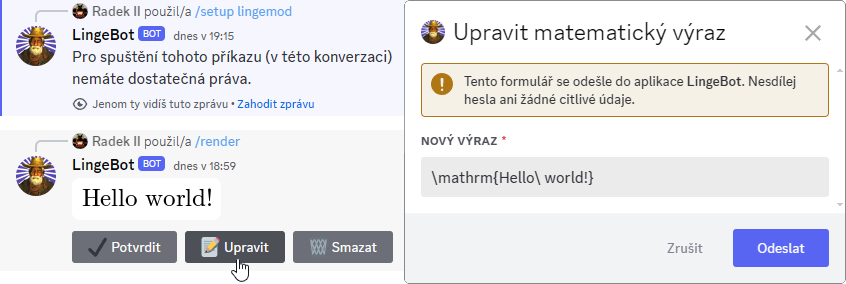
\includegraphics[width=.95\paperwidth]{img/idk}
	\end{frame}
	
	\begin{frame}\frametitle{Vykreslování matematických výrazů \texttt{/render}}
		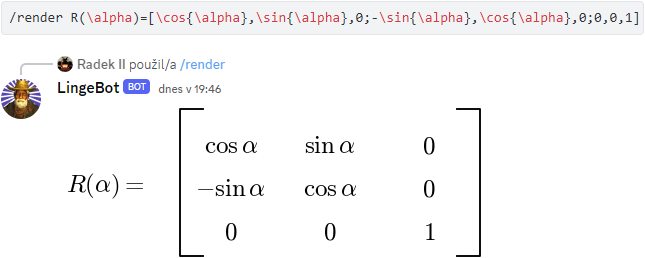
\includegraphics[width=.95\paperwidth]{img/idk2}
		\begin{itemize}
			\item Matplotlib Mathtext vs TeX
			\item Vykreslování matic a jejich zápis
			\item Rovnice s maticemi a aproximace délky výrazu
		\end{itemize}
	\end{frame}
	
	\begin{frame}[plain]\frametitle{testovací slajd bejbe}
		\makebox[\linewidth]{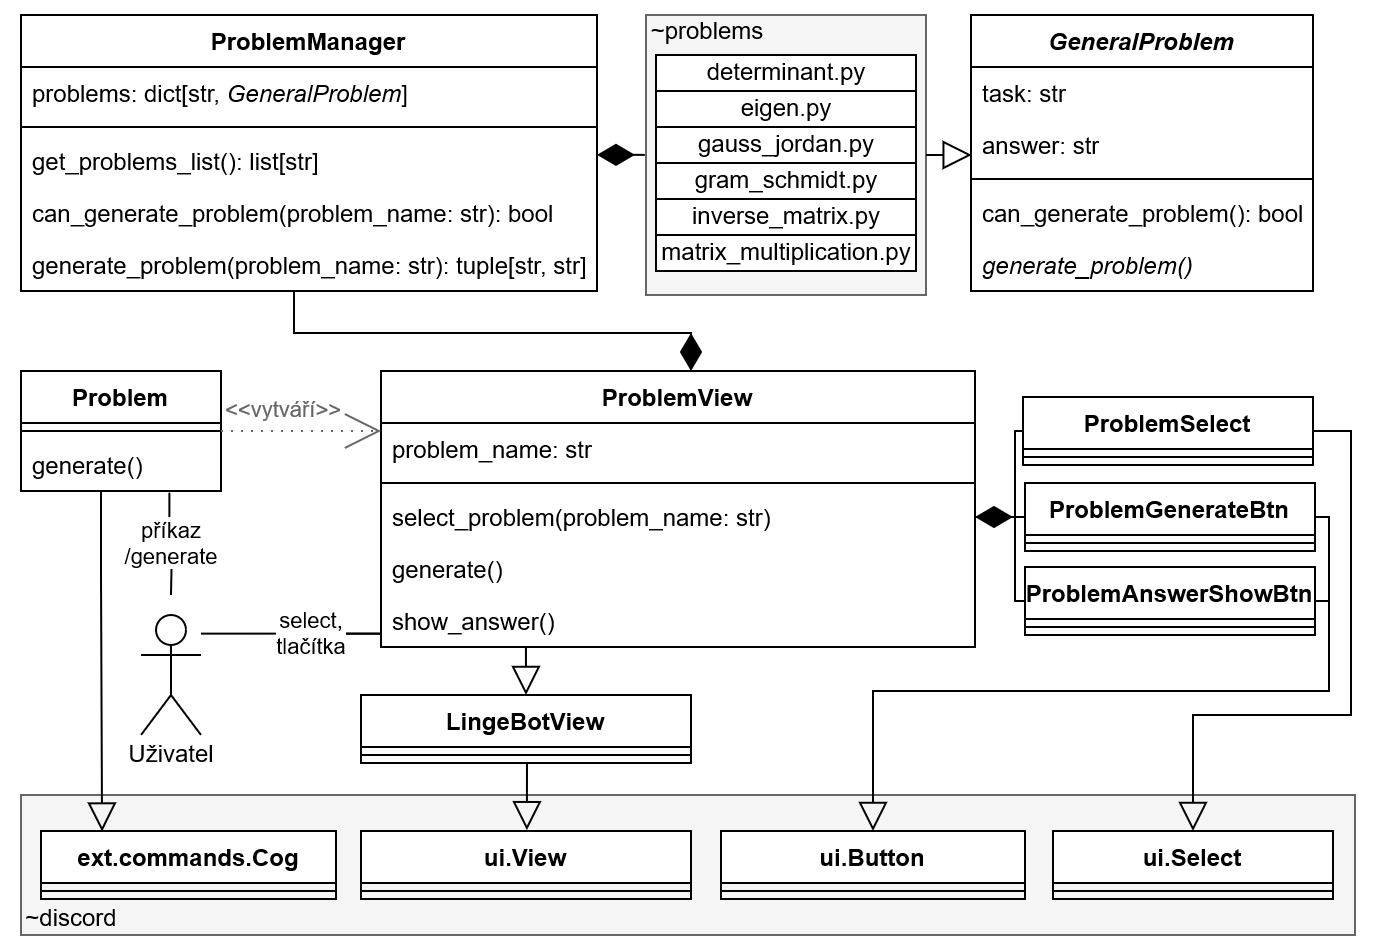
\includegraphics[width=.9\paperwidth]{img/ProblemsDiagram}}
	\end{frame}
	
	\begin{frame}\frametitle{Závěr}
		
	\end{frame}
	
	\TULendframe
\end{document}
